\documentclass{article}
\usepackage[margin=2cm]{geometry}
\usepackage{tkz-graph}
\usetikzlibrary{calc}
\usepackage{graphicx}
\usepackage{stackengine}
% DASHED LINE OF SPECIFIED LENGTH
% From morsburg at http://tex.stackexchange.com/questions/12537/
% how-can-i-make-a-horizontal-dashed-line/12553#12553
\def\dashfill{\cleaders\hbox to .6em{-}\hfill}
\newcommand\dashline[1]{\hbox to #1{\dashfill\hfil}}
\begin{document}
\savestack{\mygraph}{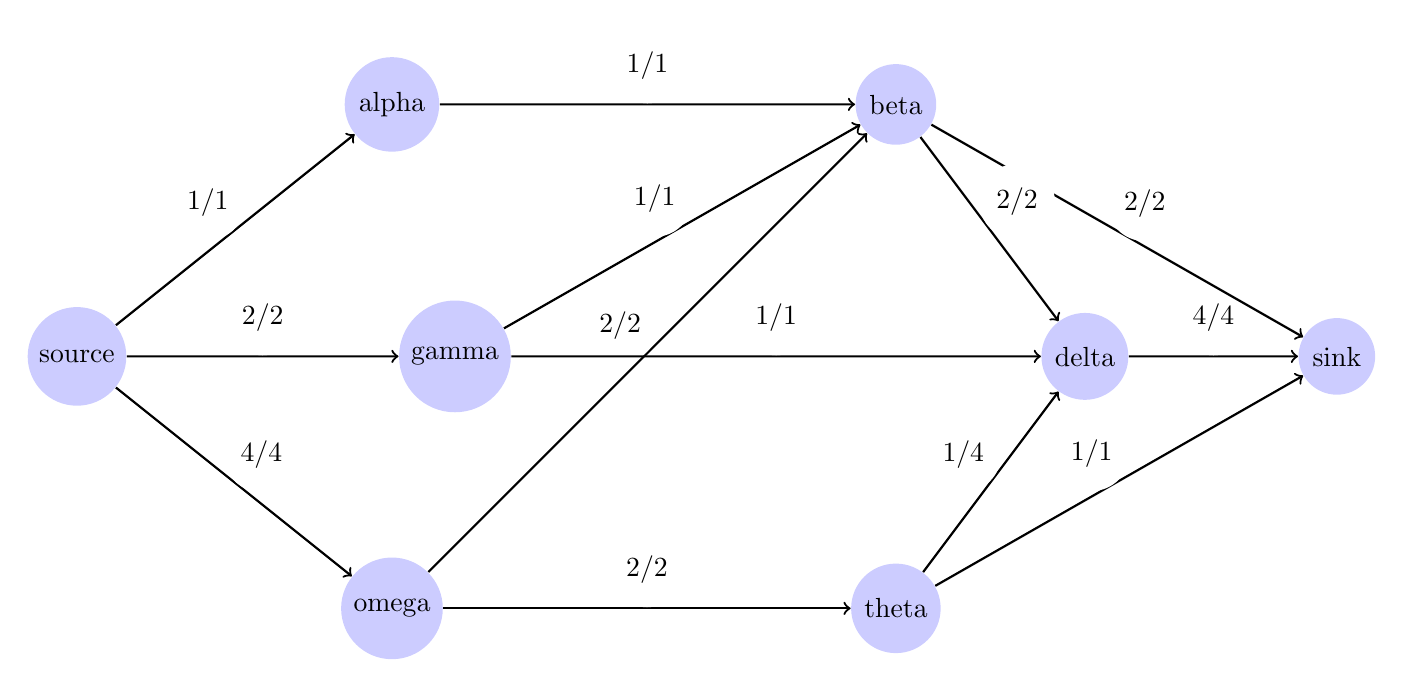
\begin{tikzpicture}
[scale=.8,auto=left,every node/.style={circle,fill=blue!20}]
\tikzset{vertex/.style = {shape=circle,draw,minimum size=1.5em}}
\tikzset{edge/.style = {->,> = latex'}}
  \node (s) at (0,5){source};
  \node (v1) at (5,9){alpha};
  \node (v4) at (13,9){beta};
  \node (v2) at (5,1){omega};
  \node (v3) at (6,5){gamma};
  \node (v5) at (13,1){theta};
  \node (v6) at (16,5){delta};
  \node (t) at (20,5){sink};
\tikzset{EdgeStyle/.style={->}}
\Edge[label=$1/1$](s)(v1);
\Edge[label=$4/4$](s)(v2);
\Edge[label=$2/2$](s)(v3);
\Edge[label=$2/2$](v2)(v4);
\Edge[label=$2/2$](v2)(v5);
\Edge[label=$1/1$](v1)(v4);
\Edge[label=$1/1$](v3)(v4);
\Edge[label=$4/4$](v6)(t);
\Edge[label=$1/1$](v5)(t);
\Edge[label=$2/2$](v4)(t);
\Edge[label=$1/4$](v5)(v6);
\Edge[label=$1/1$](v3)(v6);
\Edge[label=$2/2$](v4)(v6);
\end{tikzpicture}}
\stackinset{c}{7cm}{c}{}{\rotatebox{90}{\dashline{2in}}}{%
\stackinset{c}{-4.6cm}{c}{-1.5cm}{\rotatebox{-38}{\dashline{3.2in}}}{%
\stackinset{c}{}{c}{1cm}{\dashline{6in}}{%
\mygraph}}}
\end{document}